\documentclass{ximera}

\begin{document}
	\author{Stitz-Zeager}
	\xmtitle{Right Triangle Trigonometry}


\mfpicnumber{1}

\opengraphsfile{AppRightTrig}

\setcounter{footnote}{0}

\label{AppRightTrig}

The word `trigonometry' literally means `measuring triangles,'  so naturally most students' first introduction to trigonometry focuses on triangles.   This section focuses on \index{triangle ! right}\index{right triangle}  \textbf{right triangles}, triangles in which one angle measures $90^{\circ}$.  Consider the right triangle below, where, as usual, the  small square `$\! \! \! \! \! \! \qed$' denotes the  right angle, the  labels `$a$,' `$b$,' and `$c$'  denote the lengths of the sides of the triangle, and $\alpha$ and $\beta$ represent the (measure of) the non-right angles.  As you may recall, the side opposite the right angle is called the  \index{hypotenuse} \textbf{hypotenuse} of the right triangle.  Also note that since the sum of the measures of all angles in a triangle must add to $180^{\circ}$, we have $\alpha + \beta + 90^{\circ}= 180^{\circ}$, or $\alpha + \beta = 90^{\circ}$.  Said differently, the non-right angles in a right triangle are \textit{complements}.


\begin{center}

\begin{mfpic}[15]{-5}{5}{-5}{5}
\tlabel(0,-0.75){$a$}
\tlabel(4.75,2.25){$b$}
\tlabel(0,3){$c$}
\polyline{(3.93, 0), (3.93, 0.4), (4.33, 0.4)}
\arrow \reverse \arrow \shiftpath{(-4.330,0)} \parafcn{5, 25, 5}{2.5*dir(t)}
\arrow \reverse \arrow \shiftpath{(4.330,5)}  \parafcn{215, 265, 5}{1.5*dir(t)}
\tlabel(-1.5,0.5){$\beta$}
\tlabel(3,3){$\alpha$}
\penwd{1.25pt}
\polyline{(-4.330,0), (4.330,0), (4.330,5), (-4.330,0)}
\end{mfpic}

\end{center}

We now state and prove the most famous result about right triangles:  \index{Pythagorean Theorem}\index{Theorem ! Pythagorean} \textbf{The Pythagorean Theorem}.

%% \colorbox{ResultColor}{\bbm

\begin{theorem} \label{PythagoreanTheorem} (\textbf{The Pythagorean Theorem}) The square of the length of the hypotenuse of a right triangle is equal to the sums of the squares of the other two sides.  More specifically, if $c$ is the length of the hypotenuse of a right triangle and $a$ and $b$ are the lengths of the other two sides, then $a^2 + b^2 = c^2$.


\end{theorem}


%% \ebm}

There are several proofs of the Pythagorean Theorem,\footnote{Including one by Mentor, Ohio native \href{http://www.maa.org/press/periodicals/convergence/mathematical-treasure-james-a-garfields-proof-of-the-pythagorean-theorem}{\underline{President James Garfield}}.} but the one we choose to reproduce here showcases a nice interplay between algebra and geometry.  Consider taking four copies of the right triangle below on the left and arranging them as seen below on the right.


\begin{center}

\begin{multicols}{2}

\begin{mfpic}[22.5]{-1}{5}{-1}{5}

\arrow \reverse \arrow \shiftpath{(3,0)} \parafcn{130, 175, 5}{dir(t)}
\arrow \reverse \arrow \shiftpath{(0,4)} \parafcn{275, 300, 5}{1.5*dir(t)}
\polyline{(0, 0), (0.4, 0), (0.4, 0.4), (0, 0.4), (0,0)}

\penwd{1.25pt}
\polyline{(0,0), (3,0), (0,4), (0,0)}

\tlabel[cc](1.5,-0.5){$a$}
\tlabel[cc](-0.5,2){$b$}
\tlabel[cc](2,2){$c$}
\tlabel[cc](1.5,0.5){$\beta$}
\tlabel[cc](0.5,2){$\alpha$}
\end{mfpic}


\begin{mfpic}[20]{-1}{8}{-1}{8}

\arrow \reverse \arrow \shiftpath{(3,0)} \parafcn{130, 175, 5}{dir(t)}
\arrow \reverse \arrow \shiftpath{(7,3)} \parafcn{220, 265, 5}{dir(t)}
\arrow \reverse \arrow \shiftpath{(0,4)} \parafcn{40, 85, 5}{dir(t)}
\arrow \reverse \arrow \shiftpath{(4,7)} \parafcn{310, 355, 5}{dir(t)}

\arrow \reverse \arrow \shiftpath{(3,0)} \parafcn{5, 30, 5}{1.5*dir(t)}
\arrow \reverse \arrow \shiftpath{(7,3)} \parafcn{95, 120, 5}{1.5*dir(t)}
\arrow \reverse \arrow \shiftpath{(0,4)} \parafcn{275, 300, 5}{1.5*dir(t)}
\arrow \reverse \arrow \shiftpath{(4,7)} \parafcn{185, 210, 5}{1.5*dir(t)}



\polyline{(0, 0), (0.4, 0), (0.4, 0.4), (0, 0.4), (0,0)}
\polyline{(6.6, 0), (7, 0), (7, 0.4), (6.6, 0.4), (6.6,0)}
\polyline{(6.6, 6.6), (7, 6.6), (7, 7), (6.6, 7), (6.6, 6.6)}
\polyline{(0, 6.6), (0.4, 6.6), (0.4, 7), (0, 7), (0,6.6)}
\penwd{1.25pt}
\polyline{(0,0), (7,0), (7,7), (0,7), (0,0)}
\fillcolor[gray]{.7}
\gfill \polygon{(0,4), (3,0), (7,3), (4,7), (0,4)}
\polyline{(0,4), (3,0), (7,3), (4,7), (0,4)}
\tlabel[cc](1.5,-0.5){$a$}
\tlabel[cc](-0.5,5.5){$a$}
\tlabel[cc](5.5,7.5){$a$}
\tlabel[cc](7.5,1.5){$a$}
\tlabel[cc](5,-0.5){$b$}
\tlabel[cc](-0.5,2){$b$}
\tlabel[cc](2,7.5){$b$}
\tlabel[cc](7.5,5){$b$}

\tlabel[cc](2, 5){$c$}
\tlabel[cc](5,5){$c$}
\tlabel[cc](2,2){$c$}
\tlabel[cc](5,2){$c$}


\tlabel[cc](1.5,0.5){$\beta$}
\tlabel[cc](0.5,5.5){$\beta$}
\tlabel[cc](5.5,6.5){$\beta$}
\tlabel[cc](6.5,1.5){$\beta$}

\tlabel[cc](0.5,2){$\alpha$}
\tlabel[cc](2,6.5){$\alpha$}
\tlabel[cc](6.5,5){$\alpha$}
\tlabel[cc](5,0.5){$\alpha$}


\end{mfpic}

\end{multicols}

\end{center}

It should be clear that we have produced a large square with a side length of $(a+b)$. What is also true, but may not be obvious,  is that the shaded quadrilateral is also a square.   We can readily see the shaded quadrilateral has equal sides of length $c$.  Moreover, since $\alpha + \beta = 90^{\circ}$, we get the interior angles of the shaded quadrilateral are each $90^{\circ}$.   Hence,  the shaded quadrilateral is indeed a square.

\smallskip

We finish the proof by computing the area of the of the  large square in two ways.  First, we square the length of its side: $(a+b)^2$.  Next, we add up the areas of the four triangles, each having area $\frac{1}{2} ab$ along with the area of the shaded square, $c^2$.  Equating these to expressions gives: $(a+b)^2 = 4 \left( \frac{1}{2} ab\right)+c^2$.  Since $(a+b)^2 = a^2+2ab+b^2$ and $4 \left( \frac{1}{2} ab\right)  = 2ab$, we have $a^2+2ab+b^2 = 2ab + c^2$ or $a^2+b^2 = c^2$, as required.

It should be noted that the converse of the Pythagorean Theorem is also true.  That is if $a$, $b$, and $c$ are the lengths of sides of a triangle and $a^2+b^2 = c^2$, then $c$ the triangle is a right triangle.\footnote{We will prove this in Section \ref{TheLawofCosines} by generalizing the Pythagorean Theorem to a formula that works for \textit{all} triangles.}

\smallskip

A list of integers $(a,b,c)$  which satisfy the relationship $a^2+b^2 = c^2$ is called a  \index{Pythagorean triple}\textbf{Pythagorean Triple}.  Some of the more common triples are: $(3,4,5)$,  $(5,12,13)$, $(7,24,25)$, and $(8,15,17)$.   We leave it to the reader to verify these integers satisfy the equation $a^2+b^2 = c^2$ and suggest committing these triples to memory.

\smallskip

Next, we set about defining characteristic ratios associated with acute angles.  Given any acute angle $\theta$, we can imagine $\theta$ being an interior angle of a right triangle as seen below.   

\phantomsection
\label{righttranglediagram}

\begin{center}

\begin{mfpic}[15]{-5}{5}{-5}{5}
\arrow \reverse \arrow \shiftpath{(-4.330,0)} \parafcn{5, 25, 5}{3*dir(t)}
\tlabel(-1, 0.6){$\theta$}
\tlabel(0,-0.75){$a$}
\tlabel(4.75,2.25){$b$}
\tlabel(0,3){$c$}
\polyline{(3.93, 0), (3.93, 0.4), (4.33, 0.4)}
\penwd{1.25pt}
\polyline{(-4.330,0), (4.330,0), (4.330,5), (-4.330,0)}
\end{mfpic}

\end{center}

Focusing on the arrangement of the sides of the triangle with respect to the angle $\theta$, we make the following definitions:  the side with length $a$  is called the side of the triangle which is \index{side ! adjacent}\index{adjacent side} \textbf{adjacent} to  $\theta$ and the side with length $b$ is called the side of the triangle \index{side ! opposite}\index{opposite side}\textbf{opposite} $\theta$. As usual, the side labeled `$c$' (the side opposite the right angle) is the hypotenuse.  Using this diagram, we  define three important \index{ratios ! trigonometric}\index{trigonometric ratios} \textbf{trigonometric ratios} of $\theta$.

\smallskip

%% \colorbox{ResultColor}{\bbm

\begin{definition} \label{righttrianglesinecosinetangent}    Suppose $\theta$ is an acute angle residing in a right triangle as depicted above.

\begin{itemize}

\item  The \index{sine ! right triangle} \textbf{sine} of $\theta$, denoted $\sin(\theta)$ is defined by the ratio: $\sin(\theta) = \dfrac{b}{c}$, or $\dfrac{\text{`length of opposite'}}{\text{`length of hypotenuse'}}$.

\item  The \index{cosine ! right triangle} \textbf{cosine} of $\theta$, denoted $\cos(\theta)$ is defined by the ratio: $\cos(\theta) = \dfrac{a}{c}$, or $\dfrac{\text{`length of adjacent'}}{\text{`length of hypotenuse'}}$.

\item  The \index{tangent ! right triangle} \textbf{tangent} of $\theta$, denoted $\tan(\theta)$ is defined by the ratio: $\tan(\theta) = \dfrac{b}{a}$, or $\dfrac{\text{`length of opposite'}}{\text{`length of adjacent'}}$.\

\end{itemize}

\smallskip

\end{definition}

%% \ebm}

\smallskip

For example, consider the angle $\theta$  indicated in the triangle below on the left.  Using Definition \ref{righttrianglesinecosinetangent},  we get $\sin(\theta) = \frac{4}{5}$, $\cos(\theta) = \frac{3}{5}$, and $\tan(\theta) = \frac{4}{3}$.   One may well wonder if these trigonometric ratios we've found for $\theta$ change if the triangle containing $\theta$ changes.  For example, if we scale all the sides of the triangle below on the left by a factor of $2$, we produce the  \index{similar triangle}\index{triangle ! similar} \textbf{similar triangle} below in the middle.\footnote{That is, a triangle with the same `shape' - that is, the same angles.}  Using this triangle to compute our ratios for $\theta$, we find $\sin(\theta) = \frac{8}{10} = \frac{4}{5}$, $\cos(\theta) = \frac{6}{10} = \frac{3}{5}$, and $\tan(\theta) = \frac{8}{6}  = \frac{4}{3}$.  Note that the scaling factor, here $2$, is common to all sides of the triangle, and, hence, cancels from the numerator and denominator when simplifying each of the ratios.  

\begin{center}

\begin{multicols}{3}

\begin{mfpic}[22.5]{-1}{5}{-1}{5}

\arrow \reverse \arrow  \parafcn{5, 50, 5}{dir(t)}

\polyline{(2.6, 0), (3, 0), (3, 0.4), (2.6, 0.4), (2.6,0)}

\penwd{1.25pt}
\polyline{(0,0), (3,0), (3,4), (0,0)}

\tlabel[cc](1.5,-0.5){$3$}
\tlabel[cc](3.5,2){$4$}
\tlabel[cc](1,2){$5$}
\tlabel[cc](1.5,0.5){$\theta$}
\end{mfpic}

\begin{mfpic}[22.5]{-1}{5}{-1}{5}

\arrow \reverse \arrow  \parafcn{5, 50, 5}{dir(t)}

\polyline{(2.6, 0), (3, 0), (3, 0.4), (2.6, 0.4), (2.6,0)}

\penwd{1.25pt}
\polyline{(0,0), (3,0), (3,4), (0,0)}

\tlabel[cc](1.5,-0.5){$6$}
\tlabel[cc](3.5,2){$8$}
\tlabel[cc](1,2){$10$}
\tlabel[cc](1.5,0.5){$\theta$}
\end{mfpic}

\begin{mfpic}[22.5]{-1}{5}{-1}{5}

\arrow \reverse \arrow  \parafcn{5, 50, 5}{dir(t)}

\polyline{(2.6, 0), (3, 0), (3, 0.4), (2.6, 0.4), (2.6,0)}

\penwd{1.25pt}
\polyline{(0,0), (3,0), (3,4), (0,0)}

\tlabel[cc](1.5,-0.5){$3r$}
\tlabel[cc](3.5,2){$4r$}
\tlabel[cc](1,2){$5r$}
\tlabel[cc](1.5,0.5){$\theta$}
\end{mfpic}


\end{multicols}


\end{center}

In general, thanks to the  \href{https://en.wikipedia.org/wiki/AA_postulate}{\underline{Angle Angle Similarity Postulate}},  any two \textit{right} triangles which contain our angle $\theta$ are similar which means there is a positive constant $r$ so that the sides of the triangle are $3r$, $4r$, and $5r$ as seen above on the right.  Hence, regardless of the right triangle in which we choose to imagine $\theta$,  $\sin(\theta) = \frac{4r}{5r} = \frac{4}{5}$, $\cos(\theta) = \frac{3r}{5r} = \frac{3}{5}$, and $\tan(\theta) = \frac{4r}{3r}  = \frac{4}{3}$.  Generalizing this same argument to any acute angle $\theta$ assures us that the ratios as described in Definition \ref{righttrianglesinecosinetangent} are independent of the triangle we use.

\smallskip

Our next objective is to determine the values of $\sin(\theta)$, $\cos(\theta)$, and $\tan(\theta)$ for some of the more commonly used angles.  We begin with $45^{\circ}$.  In a right triangle, if one of the non-right angles measures $45^{\circ}$, then the other measures $45^{\circ}$ as well.  It follows that the two legs of the triangle must be congruent.  Since we may choose any right triangle containing a $45^{\circ}$ angle for our computations, we choose the length of one (hence both) of the legs to be $1$.  The Pythagorean Theorem gives the hypotenuse is:  $c^2 = 1^2+1^2 = 2$, so $c = \sqrt{2}$. (We take only the positive square root here since $c$ represents the length of the hypotenuse here, so, necessarily $c>0$.)  From this, we obtain the values below, and suggest committing them to memory. 

\begin{multicols}{2}

\begin{mfpic}[18]{-5}{5}{-5}{5}

\arrow \reverse \arrow \shiftpath{(-2.5,0)} \parafcn{5, 35, 5}{1.5*dir(t)}
\arrow \reverse \arrow \shiftpath{(2.5,5)}  \parafcn{230, 265, 5}{1.5*dir(t)}
\tlabel(-0.8, 0.4){$45^{\circ}$}
\tlabel(1.4,2.8){$45^{\circ}$}
\tlabel(0,-0.5){$1$}
\tlabel(2.75,2.25){$1$}
\tlabel[cc](-1,3){$c=\sqrt{2}$}
\polyline{(2.1, 0), (2.1, 0.4), (2.5, 0.4)}
\penwd{1.25pt}
\polyline{(-2.5,0), (2.5,0), (2.5,5), (-2.5,0)}

\end{mfpic} 

\begin{itemize}

\item  $\sin\left(45^{\circ}\right) = \dfrac{1}{\sqrt{2}} = \dfrac{\sqrt{2}}{2}$

\item  $\cos\left(45^{\circ}\right) = \dfrac{1}{\sqrt{2}} =\dfrac{\sqrt{2}}{2}$


\item  $\tan\left(45^{\circ}\right) = \dfrac{1}{1} = 1$

\end{itemize}


\end{multicols}

Note that we have `rationalized' here to avoid the irrational number $\sqrt{2}$ appearing in the denominator.  This is a common convention in trigonometry, and we will adhere to it unless extremely inconvenient.  

\smallskip

Next, we investigate $60^{\circ}$ and $30^{\circ}$ angles.  Consider the equilateral triangle below  each of whose sides measures $2$ units.  Each of its interior angles is necessarily $60^{\circ}$, so if we drop an altitude, we produce two $30^{\circ} - 60^{\circ} - 90^{\circ}$ triangles each having a base measuring $1$ unit and a hypotenuse of $2$ units.  Using the Pythagorean Theorem, we can find the height, $h$ of these triangles: $1^2+h^2 = 2^2$ so $h^2 = 3$ or $h = \sqrt{3}$.  Using these, we can find the values of the trigonometric ratios for both $60^{\circ}$ and $30^{\circ}$.  Again, we recommend committing these values to memory.

\begin{multicols}{3}
\raggedcolumns
\begin{mfpic}[15]{-5}{5}{-5}{5}
\arrow \reverse \arrow \shiftpath{(-5,-4.330)} \parafcn{5, 55, 5}{1.5*dir(t)}
\arrow \reverse \arrow \shiftpath{(0,4.330)}  \parafcn{245, 265, 5}{2.5*dir(t)}
\tlabel(-3.4,-3.75){$60^{\circ}$}
\tlabel(-1.4,0.75){$30^{\circ}$}
\tlabel(-2.5,-5.25){$1$}
\tlabel(2.5,-5.25){$1$}
\tlabel(0.25,-1){$h=\sqrt{3}$}
\tlabel[cc](-3.25,0){$2$}
\tlabel[cc](3.25,0){$2$}
\polyline{(-0.4, -4.330), (-0.4,-3.930), (0, -3.930)}
\polyline{(0.4, -4.330), (0.4,-3.930), (0, -3.930)}
\penwd{1.25pt}
\polyline{(-5,-4.330), (0,-4.330), (0,4.330), (-5,-4.330)}
\polyline{(0,4.330), (5,-4.330), (0,-4.330)}
\end{mfpic}

\begin{itemize}

\item  $\sin\left(60^{\circ}\right) = \dfrac{\sqrt{3}}{2}$

\item  $\cos\left(60^{\circ}\right) = \dfrac{1}{2}$

\item  $\tan\left(60^{\circ}\right) = \dfrac{\sqrt{3}}{1} = \sqrt{3}$

\end{itemize}

\columnbreak


\begin{itemize}

\item  $\sin\left(30^{\circ}\right) = \dfrac{1}{2}$

\item  $\cos\left(30^{\circ}\right) = \dfrac{\sqrt{3}}{2}$

\item  $\tan\left(30^{\circ}\right) = \dfrac{1}{\sqrt{3}} = \dfrac{\sqrt{3}}{3}$

\end{itemize}


\end{multicols}

Since $30^{\circ}$ and $60^{\circ}$ are complements, the side \textit{adjacent} to the $60^{\circ}$ angle is the side \textit{opposite} the $30^{\circ}$ and the side \textit{opposite}  the $60^{\circ}$ angle is the side \textit{adjacent} to the $30^{\circ}$ .  This sort of `swapping' is true of all complementary angles and will be generalized in Section \ref{MoreTrigonometricIdentities}, Theorem \ref{cofunctionidentities}.

\smallskip

Note that the values of the trigonometric ratios we have derived for $30^{\circ}$, $45^{\circ}$, and $60^{\circ}$ angles are the \textit{exact} values of these ratios. For these angles, we can conveniently express the exact values of their sines, cosines, and tangents  resorting, at worst, to using square roots.    The reader may well wonder if, for instance, we can express the exact value of, say, $\sin\left(42^{\circ}\right)$ in terms of radicals.  The answer in this case is `yes'  (see \href{https://math.la.asu.edu/~surgent/mat170/Exact_Trig_Values.pdf}{\underline{here}}), but, in general, we will not take the time to pursue such representations.\footnote{We will do a little of this in Section \ref{MoreTrigonometricIdentities}.}  Hence, if a problem requests an `exact' answer involving $\sin\left(42^{\circ}\right)$, we will leave it written as `$\sin\left(42^{\circ}\right)$'  and use a calculator to produce a suitable approximation as the situation warrants.

Our first example requires the concept of an `angle of inclination.'  The \index{angle ! of inclination} angle of inclination (or \index{angle ! of elevation} angle of elevation) of an object refers to the angle whose initial side is some kind of base-line (say, the ground), and whose terminal side is the line-of-sight to an object above the base-line.  Schematically:
\phantomsection
\label{angleofelevation}

\begin{center}

\begin{mfpic}[18]{-5}{5}{-5}{5}
\polyline{(-4.330,0), (5,0)}
\dashed \polyline{(-4.330,0), (4.330,5)}
\arrow \shiftpath{(-4.330,0)} \parafcn{5, 25, 5}{3*dir(t)}
\tlabel(-1, 0.6){$\theta$}
\tlabel[cc](0,-1){`base line'}
\plotsymbol[3pt]{Asterisk}{(4.330,5)}
\tlabel(4.5,4.5){object}
\end{mfpic} 

\smallskip

The angle of inclination from the base line to the object is $\theta$
\end{center}

\begin{example} \label{righttriangleex1} $~$

\begin{enumerate}

\item  The angle of inclination from a point on the ground 30 feet away to the top of Lakeland's Armington Clocktower\footnote{Named in honor of Raymond Q. Armington, Lakeland's Clocktower has been a part of campus since 1972.} is  $60^{\circ}$.  Find the height of the Clocktower to the nearest foot.

\item  The Americans with Disabilities Act (ADA) stipulates the incline on an accessibility ramp be $5^{\circ}$.  If a ramp is to be built so that it replaces stairs that measure 21 inches tall, how long does the ramp need to be?  Round your answer to the nearest inch.

\item  In order to determine the height of a California Redwood tree, two sightings from the ground, one 200 feet directly behind the other, are made.  If the angles of inclination were $45^{\circ}$ and $30^{\circ}$, respectively, how tall is the tree to the nearest foot?

\end{enumerate}

{\bf Solution.}

\begin{enumerate}

\item  We can represent the problem situation using a right triangle as shown below on the left.  If we let $h$ denote the height of the tower, then we have $\tan\left(60^{\circ}\right) = \frac{h}{30}$.  From this we get an exact answer of $h = 30 \tan\left(60^{\circ}\right) = 30 \sqrt{3}$ feet.  Using a calculator, we get the approximation  $51.96$ which, when rounded to the nearest foot, gives us our answer of $52$ feet.

\item  We diagram the situation below on the left using $\ell$ to represent the unknown length of the ramp.  We have $\sin\left(5^{\circ} \right)= \frac{21}{\ell}$ so that $\ell = \frac{21}{\sin\left(5^{\circ} \right)} \approx 240.95$ inches.  Hence, the ramp is $241$ inches long.

\begin{center}

\begin{multicols}{2}

\begin{mfpic}[15]{-5}{5}{-5}{5}
\arrow \shiftpath{(0,-4.330)} \parafcn{5, 55, 5}{1.5*dir(t)}
\tlabel(1.6,-3.75){$60^{\circ}$}
\tlabel(2,-5.5){$30$ ft.}
\tlabel(5.25,0){$h$ ft.}
\polyline{(4.6, -4.330), (4.6,-3.930), (5, -3.930)}
\penwd{1.25pt}
\polyline{(0,-4.330), (5,-4.330), (5,4.330), (0,-4.330)}

\end{mfpic}

\begin{mfpic}[15]{-5}{5}{-5}{5}
\arrow \shiftpath{(-5,-4.330)} \parafcn{5, 25, 5}{3*dir(t)}
\tlabel(-1.5,-3.75){$5^{\circ}$}
\tlabel(5.25,-1.83){$21$ in.}
\tlabel(0,-1){$\ell$ in.}
\polyline{(4.6, -4.330), (4.6,-3.930), (5, -3.930)}
\penwd{1.25pt}
\polyline{(-5,-4.330), (5, -4.330), (5, 0.667), (-5, -4.330)}

\end{mfpic}


\end{multicols}

\begin{multicols}{2}
Finding the height of the Clocktower

Finding the length of an accessibility ramp.

\end{multicols}

\end{center}

\item  Sketching the problem situation below, we find ourselves with two unknowns: the height $h$ of the tree and the distance $x$ from the base of the tree to the first observation point. 

\begin{center}

\begin{mfpic}[18]{-7}{5}{-5}{5}
\arrow \shiftpath{(-2.5,0)} \parafcn{5, 35, 5}{1.5*dir(t)}
\tlabel(-0.8, 0.4){$45^{\circ}$}
\tlabel(-4, 0.4){$30^{\circ}$}
\arrow \shiftpath{(-6,0)} \parafcn{5, 25, 5}{1.75*dir(t)}
\tlabel(-5,-1){$200$ ft.}
\tlabel(-1,-1){$x$ ft.}
\tlabel(2.75,2.25){$h$ ft.}
\polyline{(2.1, 0), (2.1, 0.4), (2.5, 0.4)}
\penwd{1.25pt}
\polyline{(-2.5,0), (2.5,0), (2.5,5), (-2.5,0)}
\polyline{(-6,0), (2.5,0), (2.5,5), (-6,0)}
\point[4pt]{(-2.5,0), (-6,0)}
\end{mfpic} 

Finding the height of a California Redwood
\end{center}


Luckily, we have two right triangles to help us find each unknown, as shown below. From the triangle below on the left, we get $\tan\left(45^{\circ}\right) = \frac{h}{x}$.  From the triangle below on the right, we see  $\tan\left(30^{\circ}\right) = \frac{h}{x+200}$.  


\begin{center}

\begin{multicols}{2}

\begin{mfpic}[18]{-7}{5}{-5}{5}
\arrow \shiftpath{(-2.5,0)} \parafcn{5, 35, 5}{1.5*dir(t)}
\tlabel(-0.8, 0.4){$45^{\circ}$}
\tlabel(-1,-1){$x$ ft.}
\tlabel(2.75,2.25){$h$ ft.}
\polyline{(2.1, 0), (2.1, 0.4), (2.5, 0.4)}
\penwd{1.25pt}
\polyline{(-2.5,0), (2.5,0), (2.5,5), (-2.5,0)}
\end{mfpic} 

\begin{mfpic}[18]{-7}{5}{-5}{5}
\tlabel(-4, 0.4){$30^{\circ}$}
\arrow \shiftpath{(-6,0)} \parafcn{5, 25, 5}{1.75*dir(t)}
\tlabel(-3,-1){$x+200$ ft.}
\tlabel(2.75,2.25){$h$ ft.}
\polyline{(2.1, 0), (2.1, 0.4), (2.5, 0.4)}
\penwd{1.25pt}
\polyline{(-6,0), (2.5,0), (2.5,5), (-6,0)}
\end{mfpic} 



\end{multicols}


\end{center}


Since $\tan\left(45^{\circ}\right) = 1$, the first equation gives $\frac{h}{x} = 1$, or $x = h$.  Substituting this into the second equation gives $\frac{h}{h+200} = \tan\left(30^{\circ}\right) = \frac{\sqrt{3}}{3}$.  Clearing fractions,  we get $3h = (h+200) \sqrt{3}$.  The result is a linear equation for $h$, so we  expand the right hand side and gather all the terms involving $h$ to one side.

\[ \begin{array}{rcl}

3h & = & (h+200)\sqrt{3} \\ [5pt]
3h & = & h \sqrt{3} + 200 \sqrt{3} \\ [5pt]
3h - h \sqrt{3} & = & 200 \sqrt{3} \\ [5pt]
(3-\sqrt{3}) h & = & 200 \sqrt{3} \\ [5pt]
h & = & \dfrac{200\sqrt{3}}{3-\sqrt{3}} \approx 273.20 \\ \end{array} \] 


Hence, the tree is approximately $273$ feet tall.  \qed

\end{enumerate}

\end{example} 

There are three more trigonometric ratios which are commonly used and they are defined in the same manner the ratios in Definition \ref{righttrianglesinecosinetangent} are defined.  They are listed below.

\smallskip


%% \colorbox{ResultColor}{\bbm

\begin{definition} \label{righttriangletherest}

\smallskip

Suppose $\theta$ is an acute angle residing in a right triangle as depicted on page \pageref{righttranglediagram}.

\begin{itemize}


\item  The \index{cosecant ! right triangle} \textbf{cosecant} of $\theta$, denoted $\csc(\theta)$ is defined by the ratio: $\csc(\theta) = \dfrac{c}{b}$ , or $\dfrac{\text{`length of hypotenuse'}}{\text{`length of opposite'}}$.

\item  The \index{secant ! right triangle} \textbf{secant} of $\theta$, denoted $\sec(\theta)$ is defined by the ratio: $\sec(\theta) = \dfrac{c}{a} $ , or $\dfrac{\text{`length of hypotenuse'}}{\text{`length of adjacent'}}$.

\item  The \index{cotangent ! right triangle} \textbf{cotangent} of $\theta$, denoted $\cot(\theta)$ is defined by the ratio: $\cot(\theta) = \dfrac{a}{b} $ , or $\dfrac{\text{`length of adjacent'}}{\text{`length of opposite'}}$.

\end{itemize}

\smallskip

\end{definition}

%% \ebm}


\smallskip

We practice these definitions in the following example.

\begin{example} \label{righttriangleex2}  Suppose $\theta$ is an acute angle with $\cot(\theta) = 3$.  Find the values of the remaining five trigonometric ratios:  $\sin(\theta)$, $\cos(\theta)$, $\tan(\theta)$, $\csc(\theta)$, and $\sec(\theta)$.

{\bf Solution.}  We are given $\cot(\theta) = 3 $.  So, to proceed, we construct a right triangle in which the length of the side adjacent to $\theta$ and the length of the side opposite of $\theta$ has a ratio of $3 = \frac{3}{1}$.  Note there are infinitely many such right triangles - we have produced two below for reference.  We will focus our attention on the triangle below on the left and encourage the reader to work through the details using the triangle below on the right to verify the choice of triangle doesn't matter.

\begin{multicols}{2}

\begin{mfpic}[20]{-1}{14}{-1}{5}
\tlabel(2.25, 0.25){$\theta$}
\arrow \reverse \arrow \parafcn{3, 17, 5}{2*dir(t)}
\tlabel(3,-0.5){$3$}
\tlabel(1.25,1.5){$c = \sqrt{10}$}
\tlabel(6.5,1){$1$}
\polyline{(5.6, 0), (5.6, 0.4), (6, 0.4)}
\penwd{1.25pt}
\polyline{(0,0), (6,0), (6,2), (0,0)}
\end{mfpic} 

\begin{mfpic}[20]{-1}{14}{-1}{5}
\tlabel(2.25, 0.25){$\theta$}
\arrow \reverse \arrow \parafcn{3, 17, 5}{2*dir(t)}
\tlabel(3,-0.5){$6$}
\tlabel(6.5,1){$2$}
\polyline{(5.6, 0), (5.6, 0.4), (6, 0.4)}
\penwd{1.25pt}
\polyline{(0,0), (6,0), (6,2), (0,0)}
\end{mfpic} 


\end{multicols}

From the diagram, we see immediately $\tan(\theta) = \frac{1}{3}$, but in order to determine the remaining four trigonometric ratios, we need to first find the value of the hypotenuse. The Pythagorean Theorem gives $1^2 + 3^2 = c^2$ so $c^2 = 10$ or $c = \sqrt{10}$.   Rationalizing denominators, we find $\sin(\theta) = \frac{1}{\sqrt{10}} = \frac{\sqrt{10}}{10}$, $\cos(\theta) = \frac{3}{\sqrt{10}} = \frac{3\sqrt{10}}{10}$, $\csc(\theta) = \frac{\sqrt{10}}{1} = \sqrt{10}$ and $\sec(\theta) = \frac{\sqrt{10}}{3}$.  \qed


\end{example}

While we learned all about the trigonometric ratios of $\theta$ in Example \ref{righttriangleex2}, the identity of $\theta$ remains unknown.  Since $\sin(\theta) = \frac{\sqrt{10}}{10} \approx 0.316 $ is decidedly less than $\sin\left(30^{\circ}\right) = \frac{1}{2} = 0.5$, it stands to reason that $\theta < 30^{\circ}$. It turns out the calculator can provide for us a decimal approximation of $\theta$ by way of the `$\sin^{-1}(x)$' function.  Here, the `$-1$' exponent denotes an inverse function (see Section \ref{InverseFunctions}) does \textbf{not} mean reciprocal.\footnote{That is, $\sin^{-1}(x) \neq \frac{1}{\sin(x)} $.  That being said, $(\sin(x))^{-1} = \frac{1}{\sin(x)} = \csc(x)$.}  That is, $\sin^{-1}(x)$ (read `sine-inverse of $x$') gives an angle whose sine is $x$.  Hence, we may write $\theta = \sin^{-1}\left(\frac{\sqrt{10}}{10}\right) \approx 18.43^{\circ}$.  The functions $\cos^{-1}(x)$ and $\tan^{-1}(x)$ work similarly.  Indeed, \[ \theta = \sin^{-1}\left(\frac{\sqrt{10}}{10}\right)  = \cos^{-1}\left(\frac{3 \sqrt{10}}{10}\right)  = \tan^{-1} \left( \frac{1}{3} \right),\] and the reader is encouraged to use a calculator to verify these statements.

\smallskip

Please note there is \textbf{much} more to these inverse functions than the `angle finder' description use here.\footnote{See Section \ref{TheInverseTrigonometricFunctions} for all of the pedantic details.}  That being said, we finish this section showcasing a use for the $\tan^{-1}(x)$ function below.

\begin{example}\footnote{The authors would like to thank Dan Stitz for this problem and associated graphics.} \label{roofpitchex}  The roof on the house below has a  `$6/12$ pitch'.  This means that when viewed from the side, the roof line has a rise of 6 feet over a run of 12 feet.  Find the angle of inclination from the bottom of the roof to the top of the roof. Round your answer to the  nearest hundredth of a degree.

\begin{center}

\begin{tabular}{cc}

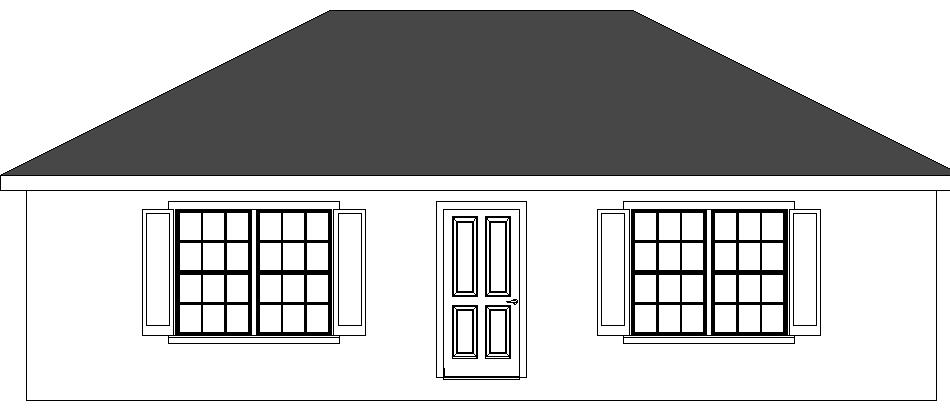
\includegraphics[width=2.75in]{./AppRightTrigGraphics/AppRightTrig01.jpg} &
\hspace{0.75in} 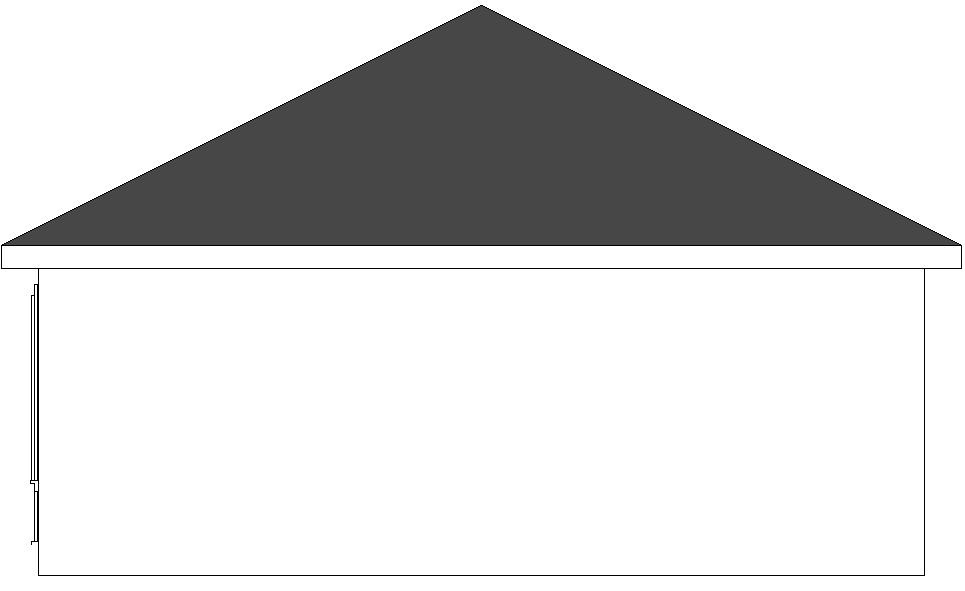
\includegraphics[width=2in]{./AppRightTrigGraphics/AppRightTrig02.jpg}  \\ 
Front View &  \hspace{0.75in} Side View \\

\end{tabular} 

\end{center}

{\bf Solution.} If we divide the side view of the house down the middle, we find that the roof line forms the hypotenuse of a right triangle with legs of length $6$ feet and $12$ feet as depicted below.  


\begin{center}

\begin{mfpic}[15]{0}{13.25}{-1}{6}
\polyline{(11.25,0), (11.25,0.75), (12,0.75)}
\arrow \reverse \arrow \polyline{(0,-1),(12,-1)}
\gclear \tlabelrect[cc](6,-1){$12$ feet}
\arrow \reverse \arrow \polyline{(13.25,0),(13.25,6)}
\gclear \tlabelrect[cc](13.25,3){$6$ feet}
\arrow \reverse \arrow \parafcn{3, 19, 5}{2.75*dir(t)}
\tlabel[cc](3.25,0.65){$\theta$}
\penwd{1.25pt}
\polyline{(0,0), (12,0), (12,6), (0,0)}
\end{mfpic}


\end{center}

The angle of inclination, $\theta$, satisfies $\tan(\theta) = \frac{6}{12} = \frac{1}{2}$.  Hence,  $\theta = \tan^{-1}\left( \frac{1}{2}\right)  \approx 26.56^{\circ}$. \qed 

\end{example}


\newpage

\subsection{Exercises}

%% SKIPPED %% \documentclass{ximera}

\begin{document}
	\author{Stitz-Zeager}
	\xmtitle{TITLE}
\mfpicnumber{1} \opengraphsfile{ExercisesforAppRightTrig} % mfpic settings added 


\label{ExercisesforAppRightTrig}
In Exercises \ref{trianglecircfirst} - \ref{trianglecirclast},  find the requested quantities.

\begin{multicols}{2} \raggedcolumns

\begin{enumerate}



\item Find $\theta$, $a$, and $c$.  \label{trianglecircfirst}

 \begin{mfpic}[15]{-5}{5}{-5}{5}

\arrow \reverse \arrow \shiftpath{(-4.330,0)} \parafcn{5, 25, 5}{3*dir(t)}
\arrow \reverse \arrow \shiftpath{(4.330,5)}  \parafcn{215, 265, 5}{1.5*dir(t)}
\tlabel(-1.25, 0.6){$\theta$}
\tlabel(0,-0.75){$9$}
\tlabel(4.75,2.25){$a$}
\tlabel(-0.5,3){$c$}
\tlabel(2.75,2.85){$60^{\circ}$}
\polyline{(3.93, 0), (3.93, 0.4), (4.33, 0.4)}
\penwd{1.25pt}
\polyline{(-4.330,0), (4.330,0), (4.330,5), (-4.330,0)}
\end{mfpic}

\vspace{.5in}
 
\item  Find $\alpha$, $b$, and $c$.

\begin{mfpic}[15]{-1}{5}{-1}{7}
\arrow \reverse \arrow \parafcn{60, 87, 5}{1.75*dir(t)}
\arrow \reverse \arrow \shiftpath{(4.357,6.709)}  \parafcn{185, 232, 5}{1.5*dir(t)}
\tlabel(0.25, 2){$34^{\circ}$}
\tlabel(2.5,3){$c$}
\tlabel(2,7){$b$}
\tlabel(-0.85,4){$12$}
\tlabel(2.25,5.75){$\alpha$}
\polyline{(0,6.304), (0.4, 6.304),  (0.4, 6.704)}
\penwd{1.25pt}
\polyline{(0,0), (0,6.709), (4.357, 6.709), (0,0)}
\end{mfpic}

\setcounter{HW}{\value{enumi}}

\end{enumerate}

\end{multicols}

\enlargethispage{.3in}

\begin{multicols}{2}

\begin{enumerate}

\setcounter{enumi}{\value{HW}}

\item  Find $\theta$, $a$, and $c$.

\begin{mfpic}[18]{-5}{5}{-5}{5}
\arrow \reverse \arrow \shiftpath{(2.5,0)} \parafcn{140, 175, 5}{1.5*dir(t)}
\arrow \reverse \arrow \shiftpath{(-2.5,5)}  \parafcn{275, 310, 5}{1.5*dir(t)}
\tlabel(-2, 2.75){$47^{\circ}$}
\tlabel(-0.5,-0.75){$6$}
\tlabel(-3.25,2.25){$a$}
\tlabel(0,3){$c$}
\tlabel(0.5,0.5){$\theta$}
\polyline{(-2.5, 0.4), (-2.1, 0.4), (-2.1, 0)}
\penwd{1.25pt}
\polyline{(-2.5, 0), (2.5,0), (-2.5,5), (-2.5,0)}
\end{mfpic}

\item Find $\beta$, $b$, and $c$.  \label{trianglecirclast}

\begin{mfpic}[18]{-6}{1}{-1}{9}
\arrow \reverse \arrow \parafcn{95, 127, 5}{1.75*dir(t)}
\arrow \reverse \arrow \shiftpath{(-5.402,6)}  \parafcn{317, 355, 5}{1.5*dir(t)}
\tlabel(-3.75, 5){$\beta$}
\tlabel(0.5,3){$2.5$}
\tlabel(-2.6,6.25){$b$}
\tlabel(-3.25,2.5){$c$}
\tlabel(-1.2,2){$50^{\circ}$}
\polyline{(0,5.6), (-0.4, 5.6),  (-0.4, 6)}
\penwd{1.25pt}
\polyline{(0,0), (0,6), (-5.402, 6), (0,0)}
\end{mfpic} 

\setcounter{HW}{\value{enumi}}

\end{enumerate}

\end{multicols}

In Exercises \ref{moretrianglecircfirst} - \ref{moretrianglecirclast}, answer the following questions assuming  $\theta$ is an angle in a right triangle.

\begin{enumerate}

\setcounter{enumi}{\value{HW}}

\item  If $\theta = 30^{\circ}$ and the side opposite $\theta$ has length $4$, how long is the side adjacent to $\theta$? \label{moretrianglecircfirst}

\item  If $\theta = 15^{\circ}$ and the hypotenuse has length $10$, how long is the side opposite $\theta$?

\item  If $\theta = 87^{\circ}$ and the side adjacent to $\theta$ has length $2$, how long is the side opposite $\theta$?

\item  If $\theta = 38.2^{\circ}$ and the side opposite $\theta$ has lengh $14$, how long is the hypoteneuse?

\item  If $\theta = 2.05^{\circ}$ and the hypotenuse has length $3.98$, how long is the side adjacent to $\theta$?

\item  If $\theta = 42^{\circ}$ and the side adjacent to $\theta$ has length $31$, how long is the side opposite $\theta$? \label{moretrianglecirclast}

\setcounter{HW}{\value{enumi}}

\end{enumerate}

In Exercises \ref{trianglesidesfirst} - \ref{trianglesideslast}, find the two acute angles in the right triangle whose sides have the given lengths.  Express your answers using degree measure rounded to two decimal places.

\begin{multicols}{3}

\begin{enumerate}

\setcounter{enumi}{\value{HW}}

\item 3, 4 and 5 \label{trianglesidesfirst}

\item 5, 12 and 13

\item 336, 527 and 625 \label{trianglesideslast}

\setcounter{HW}{\value{enumi}}

\end{enumerate}

\end{multicols}


\newpage

In Exercises \ref{findothercircfirstapprighttrig} - \ref{findothercirclastapprighttrig}, $\theta$ is an acute angle.  Use the given trigonometric ratio to find the exact values of the remaining trigonometric ratios of $\theta$.  Find a decimal approximation to $\theta$, rounded to two decimal places.

\begin{multicols}{3}

\begin{enumerate}
\setcounter{enumi}{\value{HW}}

\item $\sin(\theta) = \dfrac{3}{5}$  \label{findothercircfirstapprighttrig}
\item $\tan(\theta) = \dfrac{12}{5}$
\item $\csc(\theta) = \dfrac{25}{24}$

\setcounter{HW}{\value{enumi}}

\end{enumerate}

\end{multicols}

\begin{multicols}{3}

\begin{enumerate}

\setcounter{enumi}{\value{HW}}


\item $\sec(\theta) = 7$  \vphantom{$\dfrac{10}{\sqrt{91}}$}
\item $\csc(\theta) = \dfrac{10\sqrt{91}}{91}$ 
\item $\cot(\theta) = 23$ 

\setcounter{HW}{\value{enumi}}

\end{enumerate}

\end{multicols}

\begin{multicols}{3}

\begin{enumerate}

\setcounter{enumi}{\value{HW}}




\item  $\tan(\theta) = 2$  \vphantom{$\sqrt{5}$}
\item  $\sec(\theta) = 4$  \vphantom{$\sqrt{5}$}
\item $\cot(\theta) = \sqrt{5}$ 

\setcounter{HW}{\value{enumi}}

\end{enumerate}

\end{multicols}


\begin{multicols}{3}

\begin{enumerate}

\setcounter{enumi}{\value{HW}}


\item  $\cos(\theta) = \dfrac{1}{3}$ 

\item  $\cot(\theta) = 2$ \vphantom{$ \dfrac{1}{3}$}

\item  $\csc(\theta) = 5$ \vphantom{$ \dfrac{1}{3}$}

\setcounter{HW}{\value{enumi}}

\end{enumerate}

\end{multicols}

\begin{multicols}{3}

\begin{enumerate}

\setcounter{enumi}{\value{HW}}

\item  $\tan(\theta) = \sqrt{10}$ 
\item  $\sec(\theta) = 2\sqrt{5}$ 
\item  $\cos(\theta) = 0.4$  \vphantom{$\sqrt{10}$}  \label{findothercirclastapprighttrig}

\setcounter{HW}{\value{enumi}}

\end{enumerate}

\end{multicols}


\begin{enumerate}

\setcounter{enumi}{\value{HW}}

\item A tree standing vertically on level ground casts a 120 foot long shadow.  The angle of elevation from the end of the shadow to the top of the tree is $21.4^{\circ}$.  Find the height of the tree to the nearest foot.  With the help of your classmates, research the term \emph{umbra versa} and see what it has to do with the shadow in this problem.

\item The broadcast tower for radio station WSAZ (Home of ``Algebra in the Morning with Carl and Jeff'') has two enormous flashing red lights on it: one at the very top and one a few feet below the top.  From a point 5000 feet away from the base of the tower on level ground the angle of elevation to the top light is $7.970^{\circ}$ and to the second light is $7.125^{\circ}$.  Find the distance between the lights to the nearest foot.

\item On page \pageref{angleofelevation} we defined the angle of inclination (also known as the angle of elevation) and in this exercise we introduce a related angle - \index{angle ! of depression} the angle of depression (also known as \index{angle ! of declination} the angle of declination).  The angle of depression of an object refers to the angle whose initial side is a horizontal line above the object and whose terminal side is the line-of-sight to the object below the horizontal.  This is represented schematically below.
\label{angleofdepression}

\begin{center}

\begin{mfpic}[18]{-5}{5}{-5}{5}
\polyline{(-5,5), (4.330,5)}
\point[3pt]{(4.330,5)}
\dashed \polyline{(-4.330,0), (4.330,5)}
\reverse \arrow \shiftpath{(4.330,5)} \parafcn{185, 205, 5}{3*dir(t)}
\tlabel(0.75, 4){$\theta$}
\tlabel[cc](-1,5.5){horizontal}
\tlabel[cc](5.25,4.5){observer}
\plotsymbol[3pt]{Asterisk}{(-4.330,0)}
\tlabel(-5.0,-0.75){object}
\end{mfpic} 

\smallskip

The angle of depression from the horizontal to the object is $\theta$

\end{center}

\begin{enumerate}

\item Show that if the horizontal is above and parallel to level ground then the angle of depression (from observer to object) and the angle of inclination (from object to observer) will be congruent because they are alternate interior angles.

\item \label{sasquatchfire} From a firetower 200 feet above level ground in the Sasquatch National Forest, a ranger spots a fire off in the distance.  The angle of depression to the fire is $2.5^{\circ}$.  How far away from the base of the tower is the fire?

\item  The ranger in part \ref{sasquatchfire} sees a Sasquatch running directly from the fire towards the firetower.  The ranger takes two sightings.  At the first sighting, the angle of depression from the tower to the Sasquatch is $6^{\circ}$.  The second sighting, taken just 10 seconds later, gives the the angle of depression as $6.5^{\circ}$.  How far did the Saquatch travel in those 10 seconds?  Round your answer to the nearest foot.  How fast is it running in miles per hour? Round your answer to the nearest mile per hour.  If the Sasquatch keeps up this pace, how long will it take for the Sasquatch to reach the firetower from his location at the second sighting?  Round your answer to the nearest minute.

\end{enumerate}

\item  When I stand 30 feet away from a tree at home, the angle of elevation to the top of the tree is $50^{\circ}$ and the angle of depression to the base of the tree is $10^{\circ}$.  What is the height of the tree?  Round your answer to the nearest foot.

\item From the observation deck of the lighthouse at Sasquatch Point 50 feet above the surface of Lake Ippizuti, a lifeguard spots a boat out on the lake sailing directly toward the lighthouse.  The first sighting had an angle of depression of $8.2^{\circ}$ and the second sighting had an angle of depression of $25.9^{\circ}$.  How far had the boat traveled between the sightings?

\item A guy wire 1000 feet long is attached to the top of a tower.  When pulled taut it makes a $43^{\circ}$ angle with the ground.  How tall is the tower?  How far away from the base of the tower does the wire hit the ground?

\setcounter{HW}{\value{enumi}}

\end{enumerate}

\begin{enumerate}

\setcounter{enumi}{\value{HW}}

\item A guy wire 1000 feet long is attached to the top of a tower.  When pulled taut it touches level ground 360 feet from the base of the tower.  What angle does the wire make with the ground?  Express your answer using degree measure rounded to one decimal place.

\item At Cliffs of Insanity Point, The Great Sasquatch Canyon is 7117 feet deep.  From that point, a fire is seen at a location known to be 10 miles away from the base of the sheer canyon wall.  What angle of depression is made by the line of sight from the canyon edge to the fire?  Express your answer using degree measure rounded to one decimal place.

\item Shelving is being built at the Utility Muffin Research Library which is to be 14 inches deep.  An 18-inch rod will be attached to the wall and the underside of the shelf at its edge away from the wall, forming a right triangle under the shelf to support it.  What angle, to the nearest degree, will the rod make with the wall?

\item A parasailor is being pulled by a boat on Lake Ippizuti.  The cable is 300 feet long and the parasailor is 100 feet above the surface of the water.  What is the angle of elevation from the boat to the parasailor?  Express your answer using degree measure rounded to one decimal place.

\item  A tag-and-release program to study the Sasquatch population of the eponymous Sasquatch National Park is begun.  From a 200 foot tall tower, a ranger spots a Sasquatch lumbering through the wilderness directly towards the tower.  Let $\theta$ denote the angle of depression from the top of the tower to a point on the ground.  If the range of the rifle with a tranquilizer dart is 300 feet, find the smallest value of $\theta$ for which the corresponding point on the ground is in range of the rifle.  Round your answer to the nearest hundreth of a degree.

\item  The rule of thumb for safe ladder use states that the length of the ladder should be at least four times as long as the distance from the base of the ladder to the wall. Assuming the ladder is resting against a wall which is `plumb' (that is, makes a $90^{\circ}$ angle with the ground), determine the acute angle the ladder makes with the ground, rounded to the nearest tenth of a degree.

\setcounter{HW}{\value{enumi}}

\end{enumerate}

As you may have already noticed in working through the exercises, since the six trigonometric ratios are all defined in terms of the three sides of a right triangle, there are several relationships between them.  In Exercises \ref{rtidentityfirst} - \ref{rtidentitylast}, use the diagram on page \pageref{righttranglediagram} along with Definitions \ref{righttrianglesinecosinetangent} and \ref{righttriangletherest} to show the following relationships hold for all acute angles.\footnote{These are called trigonometric \textit{identities} and will be studied in greater detail in Section \ref{FundamentalTrigonometricIdentities}.}

\begin{multicols}{3}

\begin{enumerate}

\setcounter{enumi}{\value{HW}}

\item  $\tan(\theta) = \dfrac{\sin(\theta)}{\cos(\theta)}$ \label{rtidentityfirst}

\item  $\csc(\theta) = \dfrac{1}{\sin(\theta)}$

\item  $\sec(\theta) = \dfrac{1}{\cos(\theta)}$

\setcounter{HW}{\value{enumi}}

\end{enumerate}

\end{multicols}

For Exercises \ref{rtcofunctionfirst} - \ref{rrcofunctionlast}, it may be helpful to recall that $90^{\circ} - \theta$ is the measure of the `other' acute angle in the right triangle besides $\theta$.


\begin{multicols}{3}

\begin{enumerate}

\setcounter{enumi}{\value{HW}}

\item  $\cos(\theta) = \sin\left( 90^{\circ} - \theta \right) $ \label{rtcofunctionfirst} \label{cofunctionforeshadowing}

\item  $\csc(\theta) = \sec\left( 90^{\circ} - \theta \right) $

\item  $\cot(\theta) = \tan\left( 90^{\circ} - \theta \right) $ \label{rrcofunctionlast}

\setcounter{HW}{\value{enumi}}

\end{enumerate}

\end{multicols}

For Exercises \ref{rtpythexercisefirst} - \ref{rtpythexerciselast}, it may be helpful to remember that $a^2+b^2 = c^2$:

\begin{multicols}{3}

\begin{enumerate}

\setcounter{enumi}{\value{HW}}

\item  $(\cos(\theta))^2 + (\sin(\theta))^2 = 1$ \label{rtpythexercisefirst}

\item  $1 + (\tan(\theta))^2 = (\sec(\theta))^2$

\item  $ 1 + (\cot(\theta))^2 = (\csc(\theta))^2$ \label{rtpythexerciselast} \label{rtidentitylast}

\setcounter{HW}{\value{enumi}}

\end{enumerate}

\end{multicols}

\newpage

\subsection{Answers}

\begin{enumerate}



\item  $\theta = 30^{\circ}$, $a = 3\sqrt{3}$, $c = \sqrt{108} = 6\sqrt{3}$

\item  $\alpha = 56^{\circ}$, $b = 12 \tan(34^{\circ}) =  8.094$, $c = 12\sec(34^{\circ}) = \dfrac{12}{\cos(34^{\circ})} \approx 14.475$

\item  $\theta = 43^{\circ}$, $a = 6\cot(47^{\circ}) = \dfrac{6}{\tan(47^{\circ})} \approx 5.595$, $c = 6\csc(47^{\circ}) = \dfrac{6}{\sin(47^{\circ})} \approx 8.204$

\item  $\beta = 40^{\circ}$, $b = 2.5 \tan(50^{\circ}) \approx 2.979$, $c = 2.5\sec(50^{\circ}) = \dfrac{2.5}{\cos(50^{\circ})} \approx 3.889$

\setcounter{HW}{\value{enumi}}

\end{enumerate}

\begin{enumerate}

\setcounter{enumi}{\value{HW}}

\item  The side adjacent to $\theta$ has length $4\sqrt{3} \approx 6.928$

\item  The side opposite $\theta$ has length $10 \sin(15^{\circ}) \approx 2.588$

\item  The side opposite $\theta$ is $2\tan(87^{\circ}) \approx 38.162$

\item  The hypoteneuse has length $14 \csc(38.2^{\circ}) = \dfrac{14}{\sin(38.2^{\circ})} \approx 22.639$

\item  The side adjacent to $\theta$ has length $3.98 \cos(2.05^{\circ}) \approx 3.977$

\item  The side opposite $\theta$ has length $31\tan(42^{\circ}) \approx 27.912$

\setcounter{HW}{\value{enumi}}

\end{enumerate}

\begin{multicols}{3}

\begin{enumerate}

\setcounter{enumi}{\value{HW}}

\item $36.87^{\circ}$ and $53.13^{\circ}$
\item $22.62^{\circ}$ and $67.38^{\circ}$
\item $32.52^{\circ}$ and $57.48^{\circ}$

\setcounter{HW}{\value{enumi}}

\end{enumerate}

\end{multicols}


\begin{enumerate}

\setcounter{enumi}{\value{HW}}

\item $\sin(\theta) = \frac{3}{5}, \cos(\theta) = \frac{4}{5}, \tan(\theta) = \frac{3}{4}, \csc(\theta) = \frac{5}{3}, \sec(\theta) = \frac{5}{4}, \cot(\theta) = \frac{4}{3}$, $\theta \approx 36.87^{\circ}$

\item $\sin(\theta) = \frac{12}{13}, \cos(\theta) = \frac{5}{13}, \tan(\theta) = \frac{12}{5}, \csc(\theta) = \frac{13}{12}, \sec(\theta) = \frac{13}{5}, \cot(\theta) = \frac{5}{12}$, $\theta \approx 67.38^{\circ}$

\item $\sin(\theta) = \frac{24}{25}, \cos(\theta) = \frac{7}{25}, \tan(\theta) = \frac{24}{7}, \csc(\theta) = \frac{25}{24}, \sec(\theta) = \frac{25}{7}, \cot(\theta) = \frac{7}{24}$, $\theta \approx 73.74^{\circ}$

\item $\sin(\theta) = \frac{4\sqrt{3}}{7}, \cos(\theta) = \frac{1}{7}, \tan(\theta) = 4\sqrt{3}, \csc(\theta) = \frac{7\sqrt{3}}{12}, \sec(\theta) = 7, \cot(\theta) = \frac{\sqrt{3}}{12}$,  $\theta \approx 81.79^{\circ}$

\item $\sin(\theta) = \frac{\sqrt{91}}{10}, \cos(\theta) = \frac{3}{10}, \tan(\theta) = \frac{\sqrt{91}}{3}, \csc(\theta) = \frac{10\sqrt{91}}{91}, \sec(\theta) = \frac{10}{3}, \cot(\theta) = \frac{3\sqrt{91}}{91}$, $\theta \approx 72.54^{\circ}$

\item $\sin(\theta) = \frac{\sqrt{530}}{530}, \cos(\theta) = \frac{23\sqrt{530}}{530}, \tan(\theta) = \frac{1}{23}, \csc(\theta) = \sqrt{530}, \sec(\theta) = \frac{\sqrt{530}}{23}, \cot(\theta) = 23$, $\theta \approx 2.49^{\circ}$

\item $\sin(\theta) = \frac{2\sqrt{5}}{5}, \cos(\theta) = \frac{\sqrt{5}}{5}, \tan(\theta) = 2, \csc(\theta) = \frac{\sqrt{5}}{2}, \sec(\theta) = \sqrt{5}, \cot(\theta) = \frac{1}{2}$, $\theta \approx 63.43^{\circ}$

\item  $\sin(\theta) = \frac{\sqrt{15}}{4}, \cos(\theta) = \frac{1}{4}, \tan(\theta) = \sqrt{15}, \csc(\theta) = \frac{4\sqrt{15}}{15}, \sec(\theta) = 4, \cot(\theta) = \frac{\sqrt{15}}{15}$, $\theta \approx 75.52^{\circ}$

\item $\sin(\theta) = \frac{\sqrt{6}}{6}, \cos(\theta) = \frac{\sqrt{30}}{6}, \tan(\theta) = \frac{\sqrt{5}}{5}, \csc(\theta) = \sqrt{6}, \sec(\theta) = \frac{\sqrt{30}}{5}, \cot(\theta) = \sqrt{5}$, $\theta \approx 24.09^{\circ}$

\item $\sin(\theta) = \frac{2\sqrt{2}}{3}, \cos(\theta) = \frac{1}{3}, \tan(\theta) = 2\sqrt{2}, \csc(\theta) = \frac{3\sqrt{2}}{4}, \sec(\theta) = 3, \cot(\theta) = \frac{\sqrt{2}}{4}$, $\theta \approx 70.53^{\circ}$

\item $\sin(\theta) = \frac{\sqrt{5}}{5}, \cos(\theta) = \frac{2\sqrt{5}}{5}, \tan(\theta) = \frac{1}{2}, \csc(\theta) = \sqrt{5}, \sec(\theta) = \frac{\sqrt{5}}{2}, \cot(\theta) = 2$, $\theta \approx 26.57^{\circ}$

\item $\sin(\theta) = \frac{1}{5}, \cos(\theta) = \frac{2\sqrt{6}}{5}, \tan(\theta) = \frac{\sqrt{6}}{12}, \csc(\theta) = 5, \sec(\theta) = \frac{5\sqrt{6}}{12}, \cot(\theta) = 2\sqrt{6}$, $\theta \approx 11.54^{\circ}$

\item $\sin(\theta) = \frac{\sqrt{110}}{11}, \cos(\theta) = \frac{\sqrt{11}}{11}, \tan(\theta) = \sqrt{10}, \csc(\theta) = \frac{\sqrt{110}}{10}, \sec(\theta) = \sqrt{11}, \cot(\theta) = \frac{\sqrt{10}}{10}$, $\theta \approx 72.45^{\circ}$

\item $\sin(\theta) = \frac{\sqrt{95}}{10}, \cos(\theta) = \frac{\sqrt{5}}{10}, \tan(\theta) = \sqrt{19}, \csc(\theta) = \frac{2\sqrt{95}}{19}, \sec(\theta) = 2\sqrt{5}, \cot(\theta) = \frac{\sqrt{19}}{19}$, $\theta \approx 77.08^{\circ}$

\item $\sin(\theta) = \frac{\sqrt{21}}{5}, \cos(\theta) = \frac{2}{5}, \tan(\theta) = \frac{\sqrt{21}}{2}, \csc(\theta) = \frac{5\sqrt{21}}{21}, \sec(\theta) = \frac{5}{2}, \cot(\theta) = \frac{2\sqrt{21}}{21}$, $\theta \approx  66.42^{\circ}$

\setcounter{HW}{\value{enumi}}

\end{enumerate}

\begin{enumerate}

\setcounter{enumi}{\value{HW}}

\item The tree is about 47 feet tall.

\item The lights are about 75 feet apart.

\setcounter{HW}{\value{enumi}}

\end{enumerate}

\begin{enumerate}

\setcounter{enumi}{\value{HW}}

\item \begin{enumerate}

\addtocounter{enumii}{1}

\item The fire is about 4581 feet from the base of the tower.

\item  The Sasquatch ran $200\cot(6^{\circ}) - 200\cot(6.5^{\circ}) \approx 147$ feet in those 10 seconds. This translates to $\approx 10$ miles per hour.  At the scene of the second sighting, the Sasquatch was $\approx 1755$ feet from the tower, which means, if it keeps up this pace, it will reach the tower in about $2$ minutes.

\end{enumerate}

\setcounter{HW}{\value{enumi}}

\end{enumerate}

\begin{enumerate}

\setcounter{enumi}{\value{HW}}

\item  The tree is about 41 feet tall.

\item The boat has traveled about 244 feet.

\item  The tower is about 682 feet tall. The guy wire hits the ground about  731 feet away from the base of the tower.

\setcounter{HW}{\value{enumi}}

\end{enumerate}

\begin{multicols}{3}

\begin{enumerate}

\setcounter{enumi}{\value{HW}}

\item $68.9^{\circ}$

\item $7.7^{\circ}$

\item $51^{\circ}$

\setcounter{HW}{\value{enumi}}

\end{enumerate}

\end{multicols}

\begin{multicols}{3}

\begin{enumerate}

\setcounter{enumi}{\value{HW}}

\item $19.5^{\circ}$

\item  $41.81^{\circ}$

\item  $75.5^{\circ}$.

\setcounter{HW}{\value{enumi}}

\end{enumerate}

\end{multicols}

\end{document}


\closegraphsfile

\end{document}
